\section{Aspetti progettuali}
Il gioco in questione è stato progettato nell'ottica di un sistema
resistente ai guasti.\\
L'aspetto critico studiato maggiormente per raggiungere tale
obiettivo è stato 
senz'altro la comunicazione, pensata per
risultare robusta e allo stesso tempo in grado di fornire reattività ai
client di gioco, nonostante quest'ultimo non utilizzi uno schema
in tempo reale.

\subsection{Il gioco}
Le regole del gioco originale sono state lievemente semplificate per evitare eccessive complicazioni in fase di sviluppo, nello specifico abbiamo eliminato la meccanica dei poderi che avrebbe richiesto di strutturare dei meccanismi di valutazione complessi.

La logica del gioco \`e divisa in due strati paralleli, quello ``fisico'' rappresentato dal tabellone che viene man mano creato e descrive la condizione esatta del tabellone di gioco e quello ``logico'' composto dagli elementi del paesaggio, che ne valuta lo stato ed informa lo strato fisico del completamento degli elementi.

I due strati agiscono nelle due fasi del turno di un giocatore: lo strato fisico controlla che sia possibile piazzare la tessera pescata dove desidera il giocatore, garantendo che non venga violata la continuit\`a del paesaggio; lo strato logico controlla la propriet\`a dei vari elementi del paesaggio presenti sulla tessera appena posizionata e permette o meno il piazzamento dei meeple, dopo di ch\`e aggiorna i punteggi dei giocatori se rileva il completamento di un elemento di paesaggio.\\

Per valutare il completamento dei tre diversi elementi di paesaggio considerati vengono utilizzate tre tecniche specifiche:
\begin{description}
	\item[Monasteri] \hfill \\
		sono completi quando tutte le otto tessere adiacenti sono state piazzate, \`e quindi sufficiente contare il numero dei vicini.
	\item[Strade] \hfill \\
		sono complete quando hanno incroci o citt\`a che le racchiudono, vengono contate quindi le tessere appartenenti alla strada contenenti questi due elementi, quando sono 2 la strada \`e completa\footnote{Unico caso speciale \`e quando la strada si chiude su se stessa, in questa circostanza risulta completa.}.
	\item[Città] \hfill \\
		sono complete quando tutto il muro di cinta \`e chiuso e non sono presenti ``buchi'' all'interno, viene quindi tenuto il conto di quanti lati aperti sono rimasti su tutto il confine della citt\`a, quando questo numero scende a zero l'elemento \`e completo.
\end{description}

\subsection{La comunicazione}
L'aspetto principale dell'intero sistema risulta l'architettura paritaria
della rete, questa \`e stata progettata utilizzando una topologia token
ring. Questo tipo di topologia fa in modo che il gioco possieda un
\textbf{ordine} tra i vari giocatori basato su un tiro di dado come si farebbe
in una partita reale.\\
Come appena introdotto, la rete \`e stata inizialmente pensata come un \emph{token ring}, il
problema di questo approccio per\`o risulta nell'aggiornamento dello schema di
gioco: se la rete fosse completamente strutturata ad anello i pacchetti dovrebbero
percorrerlo interamente per giungere a tutti i giocatori, oppure aspettare
un intero turno di gioco per giungere al sistema di aggiornamento, complicando
inutilmente il sistema.\\
Per questi motivi \`e stata successivamente scelta una topologia \emph{completamente connessa}: anche se lo
schema di gioco non presenta particolari requisiti di latenza, tutti i nodi
contatteranno ogni volta il possessore del turno, il quale, terminata la sua
azione, restituir\`a il controllo al nodo richiedente che potr\`a aggiornare il suo
stato locale.\\

\begin{figure}[H]
\begin{minipage}{.5\textwidth}
\centering
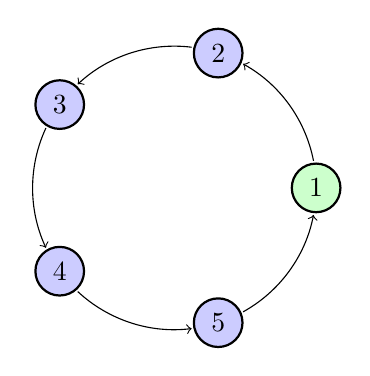
\begin{tikzpicture}[->,
	main node/.style={circle,draw,thick,fill=blue!20,minimum size=4mm},
	leader node/.style={circle,draw,thick,fill=green!20,minimum size=4mm}
]

	\def \n {5};
	\def \r {1.8cm};
	\def \m {11};

	\draw[->] (\m:\r) arc ({\m}:{360/\n -\m}:\r);

	\foreach \s in {2,...,\n} {
		\draw[->] ({360/\n * (\s-1) + \m}:\r) arc ({360/\n * (\s-1) + \m}:{360/\n * (\s) -\m}:\r);
		\node[main node] at ({360/\n * (\s-1)}:\r) {$\s$};
	}
	\node[leader node] at (0:\r) {1};
\end{tikzpicture}
\end{minipage}
\begin{minipage}{.5\textwidth}
\centering
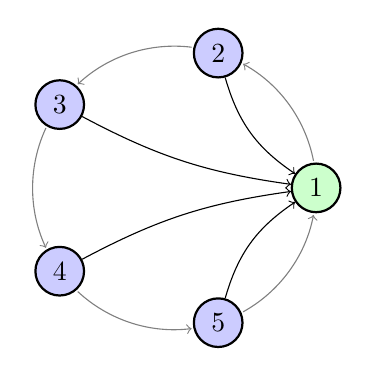
\begin{tikzpicture}[->,
	main node/.style={circle,draw,thick,fill=blue!20,minimum size=4mm},
	leader node/.style={circle,draw,thick,fill=green!20,minimum size=4mm}
]

	\def \n {5};
	\def \r {1.8cm};
	\def \m {11};

	\draw[->,gray] (\m:\r) arc ({\m}:{360/\n -\m}:\r);

	\foreach \s in {2,...,\n} {
		\draw[->,gray] ({360/\n * (\s-1) + \m}:\r) arc ({360/\n * (\s-1) + \m}:{360/\n * (\s) -\m}:\r);
		\node[main node] at ({360/\n * (\s-1)}:\r) (\s) {$\s$};
	}
	\node[leader node] at (0:\r) (L) {1};

	\draw[->] (2) to[bend right=20] (L);
	\draw[->] (3) to[bend right=10] (L);
	\draw[->] (4) to[bend left=10] (L);
	\draw[->] (5) to[bend left=20] (L);
\end{tikzpicture}
\end{minipage}
\caption{\small{Tipologia token ring (sinistra) e tipologia completamente
connessa (destra).}}
\end{figure}
La tolleranza ai guasti di tipo crash \`e quindi stata progettata in
quest'ottica: ogni nodo potr\`a accorgersi del crash di un altro giocatore
all'istante (o al momento dell'interrogazione), e riconfigurer\`a l'ordine
dell'anello in maniera appropriata.


\begin{figure}[H]
	\begin{minipage}{0.45\textwidth}
		\centering
		\begin{tikzpicture}[->,
			main node/.style={circle,draw,thick,fill=blue!20,minimum size=4mm},
			crashed node/.style={forbidden sign,draw,thick,fill=red!50,minimum size=4mm}
			]

			\def \n {5};
			\def \r {1.8cm};
			\def \m {11};

			\draw[->,gray] (\m:\r) arc ({\m}:{360/\n -\m}:\r);

			\foreach \s in {2,...,\n} {
				\draw[->,gray] ({360/\n * (\s-1) + \m}:\r) arc ({360/\n * (\s-1) + \m}:{360/\n * (\s) -\m}:\r);
				\node[main node] at ({360/\n * (\s-1)}:\r) (\s) {$\s$};
			}
			\node[crashed node] at (0:\r) (L) {1};

			\draw[->] (2) to[bend right=20] (L);
			\draw[->] (3) to[bend right=10] (L);
			\draw[->] (4) to[bend left=10] (L);
			\draw[->] (5) to[bend left=20] (L);
		\end{tikzpicture}
	\end{minipage}
	\begin{minipage}{0.45\textwidth}
		\centering
		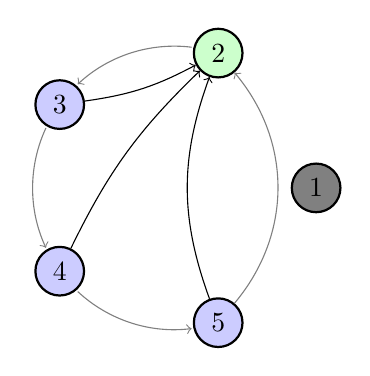
\begin{tikzpicture}[->,
			main node/.style={circle,draw,thick,fill=blue!20,minimum size=4mm},
			crashed node/.style={circle,draw,thick,fill=gray,minimum size=4mm},
			leader node/.style={circle,draw,thick,fill=green!20,minimum size=4mm}
			]

			\def \n {5};
			\def \r {1.8cm};
			\def \m {11};


			\draw[->,gray] ({360/\n * (2-1) + \m}:\r) arc ({360/\n * (2-1) + \m}:{360/\n * (2) -\m}:\r);
			\node[leader node] at ({360/\n * (2-1)}:\r) (2) {$2$};
			\draw[->,gray] ({360/\n * (3-1) + \m}:\r) arc ({360/\n * (3-1) + \m}:{360/\n * (3) -\m}:\r);
			\node[main node] at ({360/\n * (3-1)}:\r) (3) {$3$};
			\draw[->,gray] ({360/\n * (4-1) + \m}:\r) arc ({360/\n * (4-1) + \m}:{360/\n * (4) -\m}:\r);
			\node[main node] at ({360/\n * (4-1)}:\r) (4) {$4$};
			\node[main node] at ({360/\n * (5-1)}:\r) (5) {$5$};

			\draw[->,gray] (5) to [bend right=40] (2);

			\node[crashed node] at (0:\r) (L) {1};
			\draw[->] (3) to[bend right=10] (2);
			\draw[->] (4) to[bend left=10] (2);
			\draw[->] (5) to[bend left=20] (2);
		\end{tikzpicture}
	\end{minipage}
	\caption{\small{Riconfigurazione dei client dovuta ad un crash}}
\end{figure}

